\section{Animals dataset}

The \textsf{animals} dataset consists of binary values which are the answers to questions such as
"is warm-blooded?", "has lungs?", etc. There are in total 102 such questions, which make up the features, and
33 animal categories, which are the nodes. Figure~\ref{fig:animals} shows the results of estimating the
graph Laplacian of the \textsf{animals} dataset using the \textsf{GGL} algorithm with $\alpha = 0.1$ and
the proposed \textsf{SGL} algorithm with $\beta = 1/2$ and $\alpha = 10^{-1}$. The input for all the algorithms
is the sample covariance matrix plus an identity matrix scaled by $1/3$ (see Elgimez paper for an explanation of
the input).

The evaluation of the estimated graphs is done by natural intuition, i.e., we expect that similar animals
such as (\textit{ant}, \textit{cockroach}), (\textit{bee}, \textit{butterfly}), and
(\textit{trout}, \textit{salmon}), would be clustered together, while presently virtually zero connection to
other (group of) animals. Under this sense, it can be seen that the \textsf{SGL} algorithm yields a more intutive
graph than the ones learned by \textsf{GGL} and \textsf{Glasso}.

\begin{figure}[!htb]
    \centering
    \begin{subfigure}[b]{0.475\textwidth}
      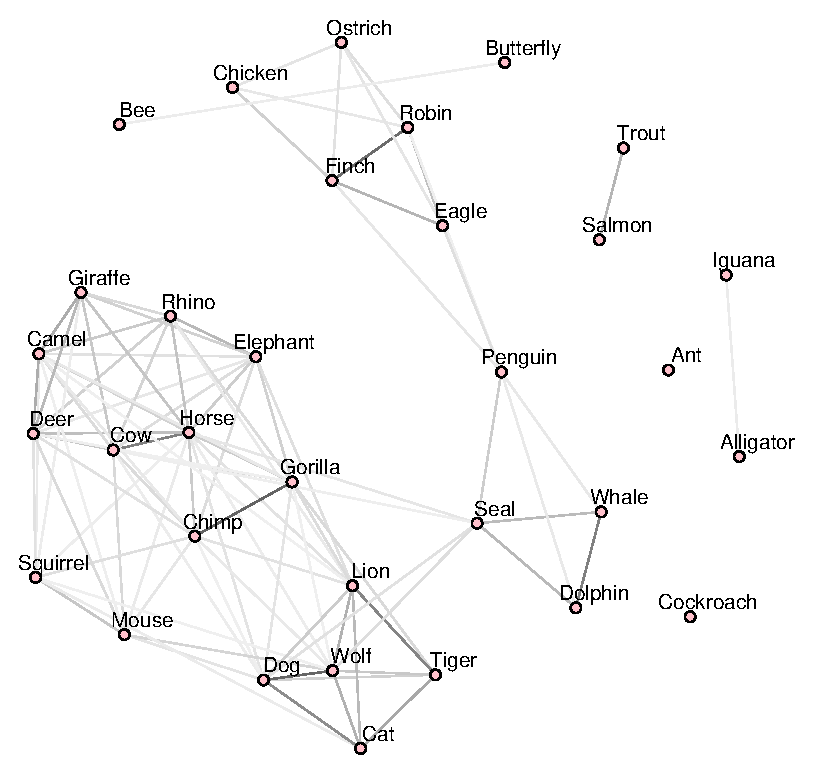
\includegraphics[width=\textwidth]{animals/latex/figures/animals_graph_ggl_alpha01.eps}
      \caption{\textsf{GGL}$(\alpha = 10^{-1})$.}
    \end{subfigure}
    ~
    \begin{subfigure}[b]{0.475\textwidth}
      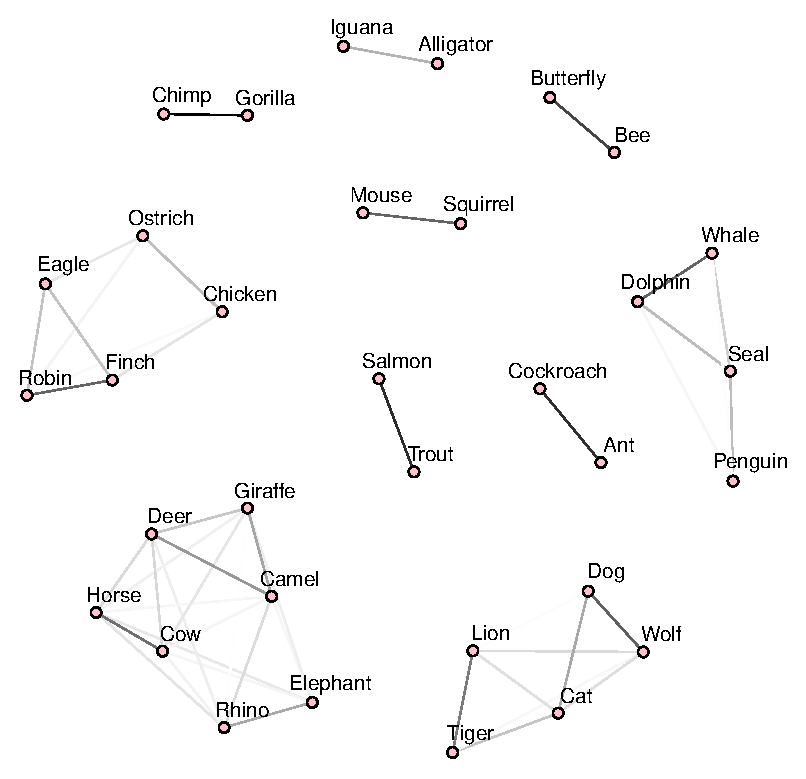
\includegraphics[width=\textwidth]{animals/latex/figures/animals_graph_k10.eps}
      \caption{\textsf{SGL}($\beta = 1/2$, $\alpha = 10^{-1}$, $K = 10$).}
    \end{subfigure}\\
    \begin{subfigure}[b]{0.475\textwidth}
      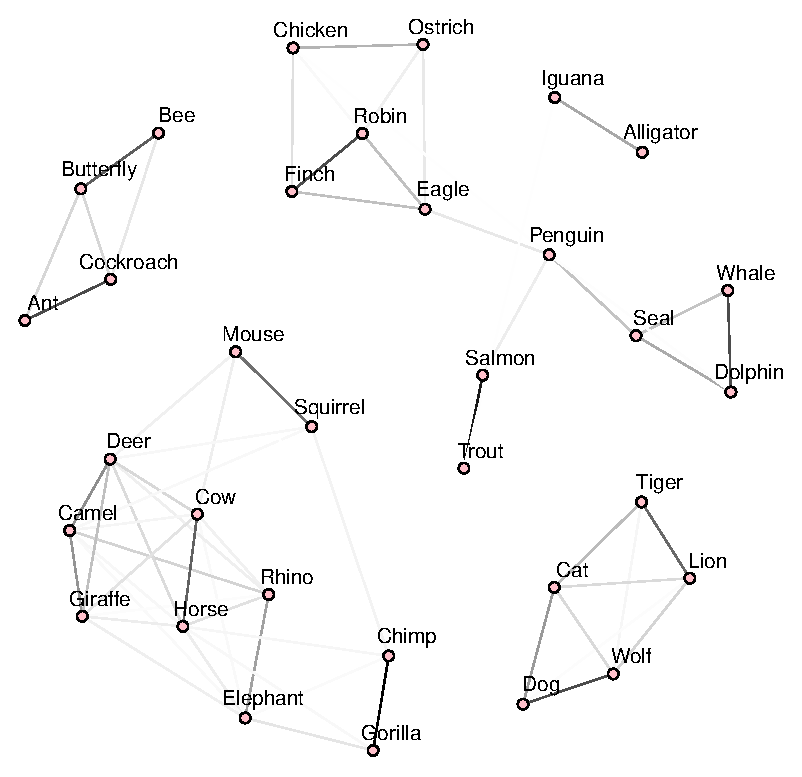
\includegraphics[width=\textwidth]{animals/latex/figures/animals_graph_k1.eps}
      \caption{\textsf{SGL}($\beta = 1/2$, $\alpha = 10^{-1}$, $K = 1$).}
    \end{subfigure}
    ~
    \begin{subfigure}[b]{0.475\textwidth}
      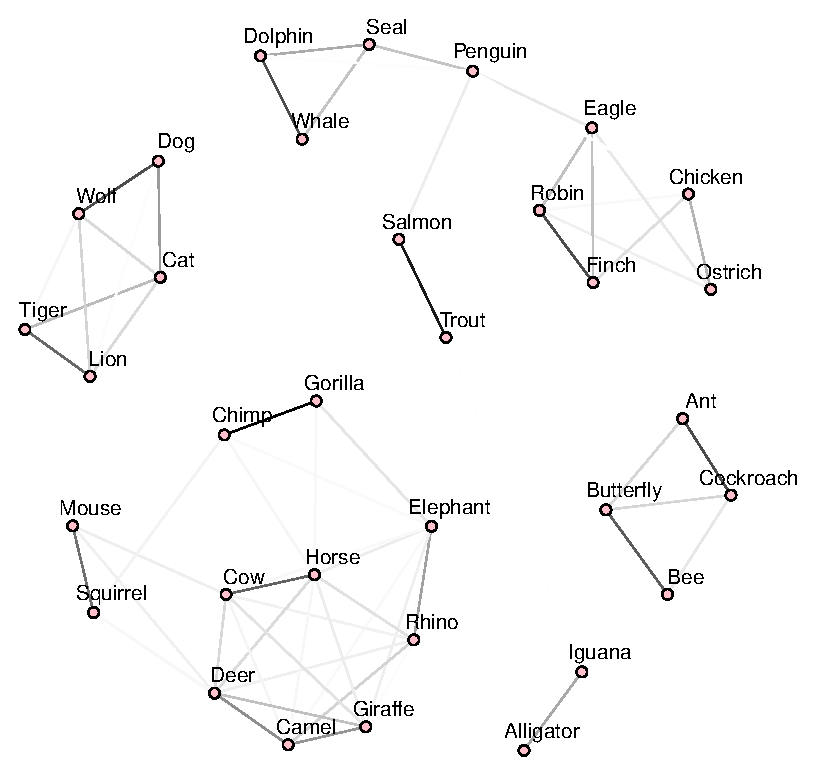
\includegraphics[width=\textwidth]{animals/latex/figures/animals_graph_k4.eps}
      \caption{\textsf{SGL}($\beta = 1/2$, $\alpha = 10^{-1}$, $K = 4$).}
    \end{subfigure}
    %~
    %\begin{subfigure}[b]{0.475\textwidth}
    %  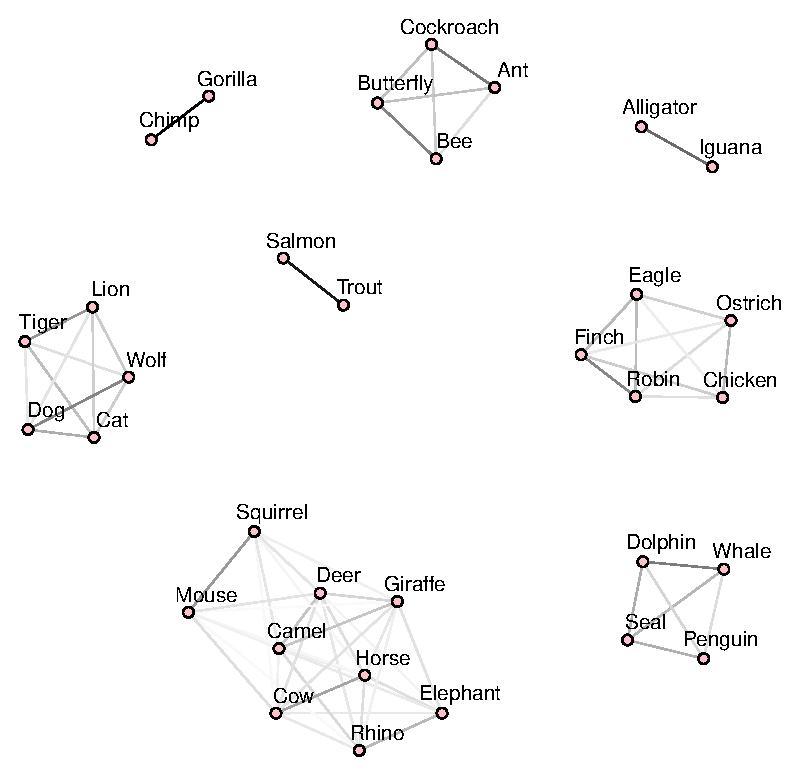
\includegraphics[width=\textwidth]{animals/graphs_for_different_k/animals_graph_k8.eps}
    %  \caption{\textsf{SGL} with $\beta = 1/2$ and $K = 8$.}
    %\end{subfigure}
    \caption{Learning the connectivity of the \textsf{animals} dataset for different values of $K$.}
    \label{fig:animals}
\end{figure}

\begin{figure}
  \centering
  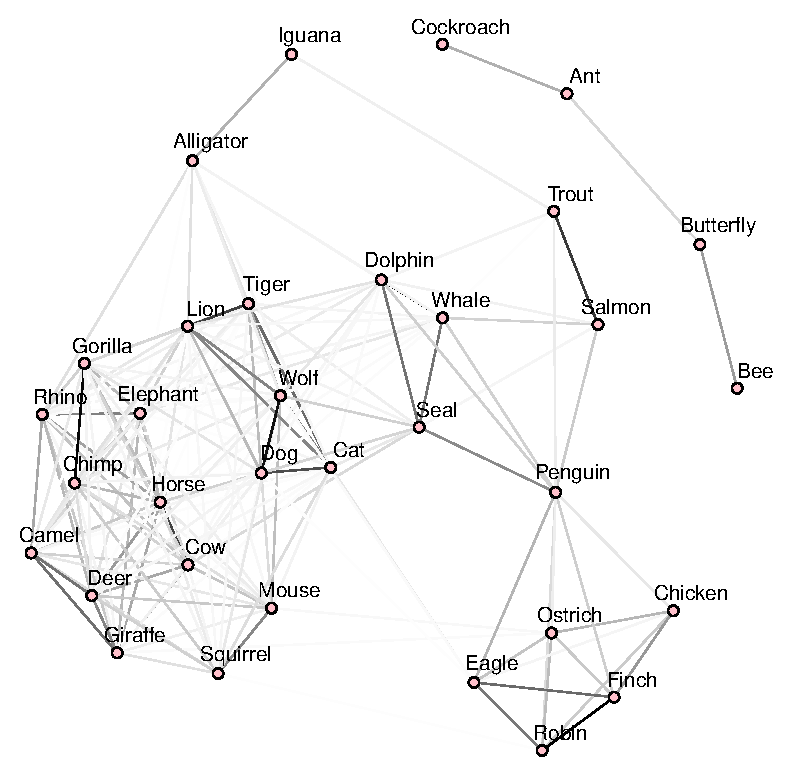
\includegraphics[width=.475\textwidth]{animals/latex/figures/animals_glasso.eps}
  \caption{Learning the connectivity of the \textsf{animals} dataset with \textsf{GLasso}.
           Regularization parameter $\alpha = 0.05618$.}
  \label{fig:animals-glasso}
\end{figure}
